\section{ Frame content analysis }

With the hypothesis that videos with majority of frames to be faces, have a greater probability to gain bigger engagement like repost and likes, we explore these videos for ontological clues about what kind of description is prevalent amongst popular videos. For this analysis, we chose the popular image ontology and sentiment analysis method called DeepSentibank \cite{chen2014deepsentibank} which is a variant of Sentibank \cite{SentiBank} by Boroth et.al, that uses deep convolutional neural networks \cite{hinton2012improving} to train a classifier which classifies images into a set of 2089 classes. Each class essentially is a ontological description that contains one adjective and a noun which describes the image. This method gives a very accessible way to understand a higher level sentiment about a particular image. We use DeepSentibank on all the face frames extracted from videos. We then trained a simple Support vector regression on the dataset of face frames to understand if there is any correlation, and if there is which are the dominant ontological adjective noun classes. This exercise was performed for both Instagram selfies and video selfie frames. Interestingly, the vine frames a larger correlation of 0.32 for likes and 0.3 for reposts, as compared with Instagram selfies popularity of 0.2 correlation. We plotted the dominant regression coefficients for all the three in figure \ref{rig:regression_coeff} to observe similar trends amongst all three. The adjective noun pairs however are different. Instagram selfies yield ANPs which are predominantly of positive sentiment, where as vine has a very mixed set. The higher correlation value shows a pattern might emerge at a higher abstraction using which prediction of reposts and likes for a video selfie vine could be possible. 
 \begin{figure}
\centering
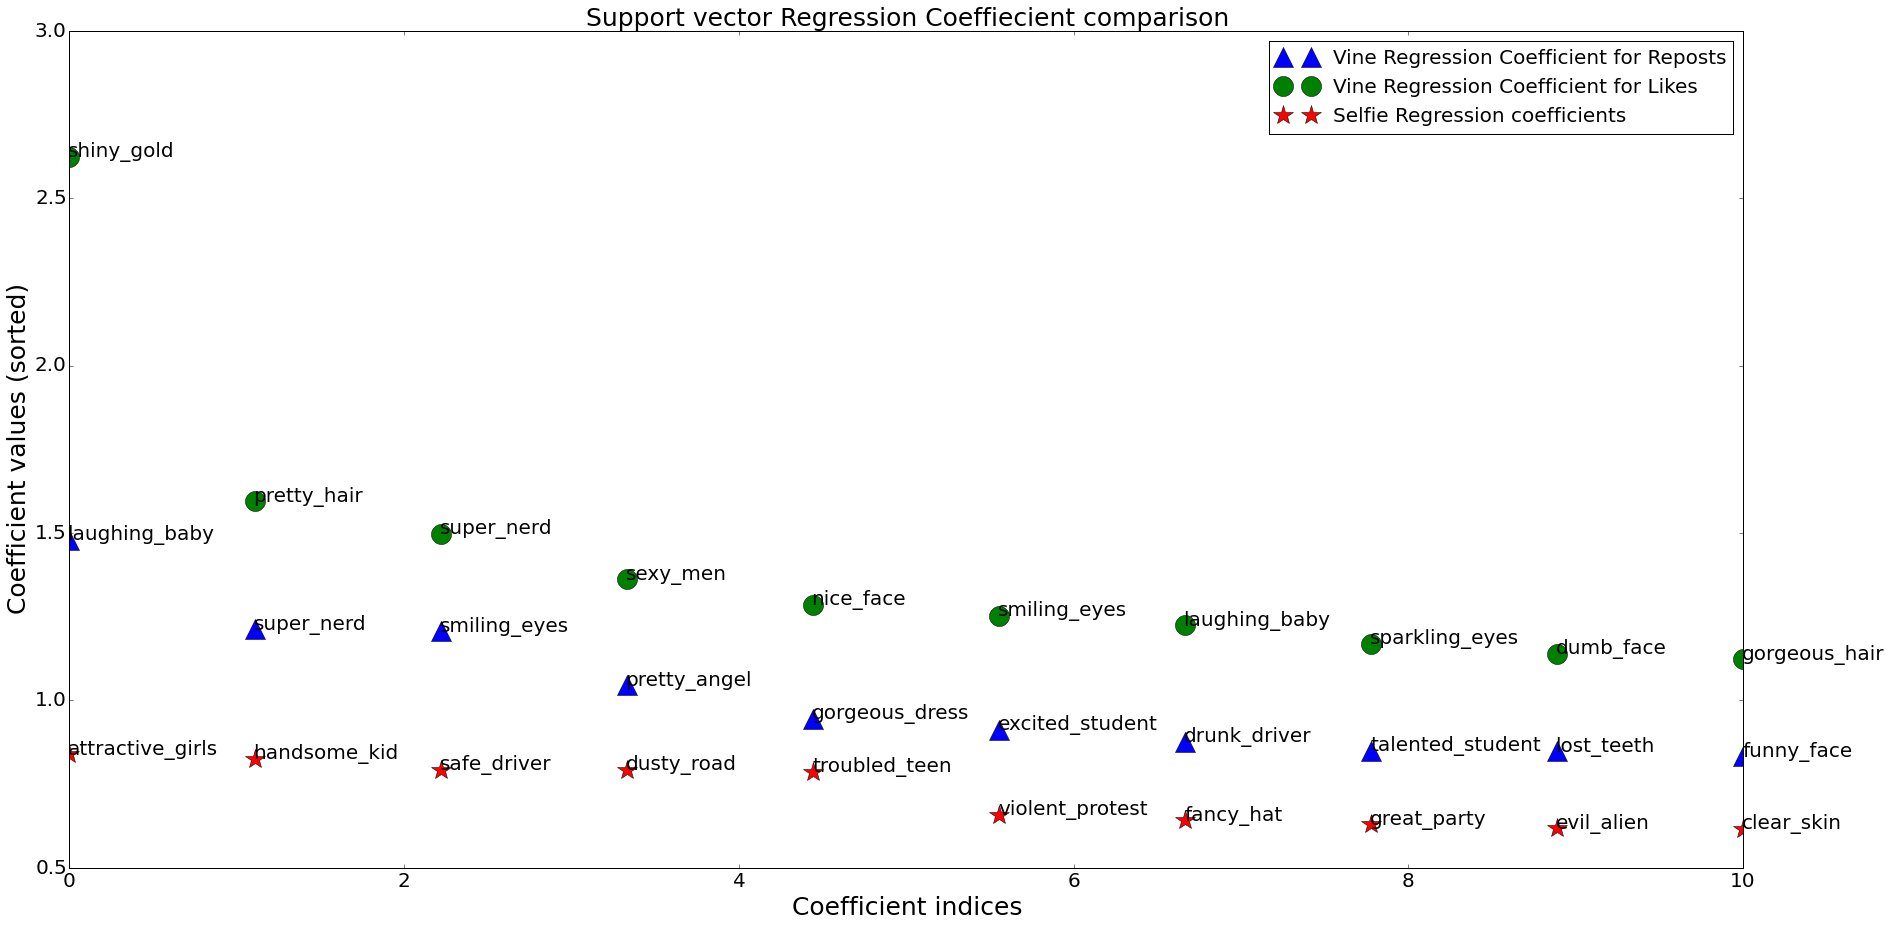
\includegraphics[width=\columnwidth]{plots/regression_coeff}
\caption{\textbf{ Top 10  Support Vector regression coefficients for Instagram selfies , Vine Likes and Vine reposts}}
\label{fig:regression_coeff}
\end{figure}
